\documentclass{article}
\usepackage{listings}
\usepackage{xcolor}

\title{The Longest Path}
\author{Do Viet Anh BI12-024}

\maketitle

\begin{document}

\lstset{language=Python,
        basicstyle=\ttfamily\footnotesize,
        breaklines=true,
        keywordstyle=\color{blue},
        stringstyle=\color{red},
        commentstyle=\color{green},
        showstringspaces=false,
        numbers=left,
        numberstyle=\tiny,
        frame=single,
        captionpos=b}

\section{Explanation of Mapper and Reducer}

\subsection{Mapper (find\_files function)}
The \texttt{find\_files} function takes two parameters: \texttt{file\_name} (the name of the file to search for) and \texttt{search\_path} (the directory path to start the search from). It works as follows:
\begin{itemize}
    \item It initializes an empty list \texttt{found\_file\_paths} to store the paths of the found files.
    \item It then iterates through each directory and subdirectory starting from \texttt{search\_path} using \texttt{os.walk()}.
    \item For each directory, it checks all the files within that directory.
    \item If a file with the name \texttt{file\_name} is found, its full path is appended to the \texttt{found\_file\_paths} list.
    \item Finally, it returns the list of found file paths.
\end{itemize}

\subsection{Reducer}
In the context of code, the reducer can be considered as the part of the code that follows the mapper function. After calling \texttt{find\_files}, the code checks if any files were found.

\section{Results}

Here are the results:

\begin{figure}[h]
  \centering
  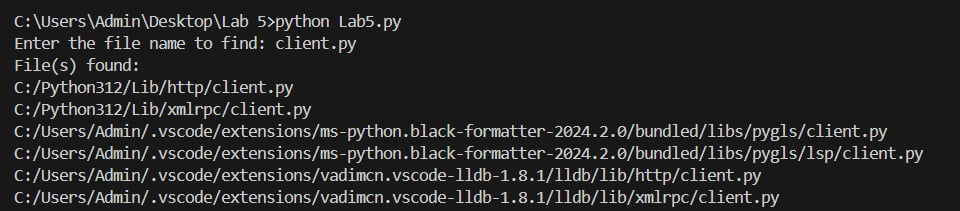
\includegraphics[width=0.8\textwidth]{lab5-1.png}
\end{figure}

\begin{figure}[h]
  \centering
  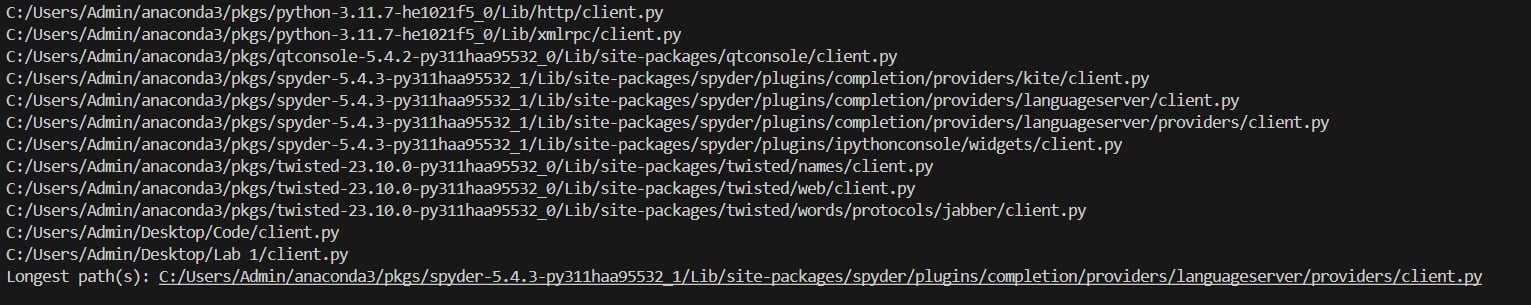
\includegraphics[width=0.8\textwidth]{lab5-2.png}
\end{figure}

\end{document}
